\documentclass[article,A4,11pt]{llncs}%
\usepackage[T1]{fontenc}
\usepackage{amsmath}
\usepackage{amssymb}
\usepackage{fullpage, graphicx, url}

\usepackage{epsf,times}
\usepackage{amsfonts}
\usepackage{graphicx}
\usepackage{mathrsfs}
\usepackage{wrapfig}

\usepackage{color}
\usepackage{amsmath,mathrsfs,bm}
\usepackage{cases}
\usepackage{subfig}
\usepackage{multicol}
\usepackage{tabularx}

% DIMIER
\usepackage[T1]{fontenc}
%\newcommand{\tmname}[1]{\textsc{#1}}
%\newcommand{\tmop}[1]{\ensuremath{\operatorname{#1}}}
%\newcommand{\tmsamp}[1]{\textsf{#1}}
%\newcommand{\tmtextsc}[1]{{\scshape{#1}}}
%\newcommand{\tmtextsl}[1]{{\slshape{#1}}}
%\newcommand{\tmtexttt}[1]{{\ttfamily{#1}}}



\leftmargin=0.2cm
\oddsidemargin=1.2cm
\evensidemargin=0cm
\topmargin=0cm
\textwidth=15.5cm
\textheight=21.5cm
\pagestyle{plain}
\setlength{\columnsep}{20pt}


\def\m{\mathbf{m}}
\def\H{\mathbf{H}}
\def\E{\mathbf{E}}
\newcommand{\vepsi}{{\varepsilon}}
\def\hnorm#1#2{\vert\,#1\,\vert_{#2}}
\newcommand{\R}{{\mathbb R}}
\newcommand{\Sph}{{\mathbb S}}
\def\x{\mathbf{x}}
\def\hvec{\overline{\mathbf{h}}}
\def\evec{\overline{\mathbf{e}}}

\DeclareMathAlphabet{\mathpzc}{OT1}{pzc}{m}{it}
%\leftmargin=0cm
%\oddsidemargin=1cm
%\textwidth=14cm
%\pagestyle{plain}

\newcommand{ \etal}{\mbox{\emph{et al. }}}

\newcommand\vect[1]{\mbf{#1}}
\newcommand{\mbf}[1]{\mbox{\boldmath$#1$}} 
\newcommand{\RC}[1]{#1 $\times$ #1 $\times$ #1}
\def\um{$\mu$m}
\def\C{$^{\circ}\mathrm{C}$}

\def\clovek#1{\noindent\bgroup\vbox{\noindent#1}\egroup\vskip1em}

% DEFINITION OF CUSTOM FONT SIZE
\newcommand{\customfontA}{\fontsize{50}{55}\selectfont}
\newcommand{\customfontB}{\fontsize{14.4}{20}\selectfont}
\newcommand{\customfontC}{\fontsize{30}{35}\selectfont}

% TO INPUT BACKGROUND IMAGE
\usepackage{eso-pic}
\newcommand\BackgroundPic{
\put(0,0){
\parbox[b][\paperheight]{\paperwidth}{%
\vfill
\centering
%\includegraphics[width=\paperwidth,height=\paperheight]{background_plzen.jpg}%
%\includegraphics[width=\paperwidth,height=\paperheight]{background_tmp.jpg}%
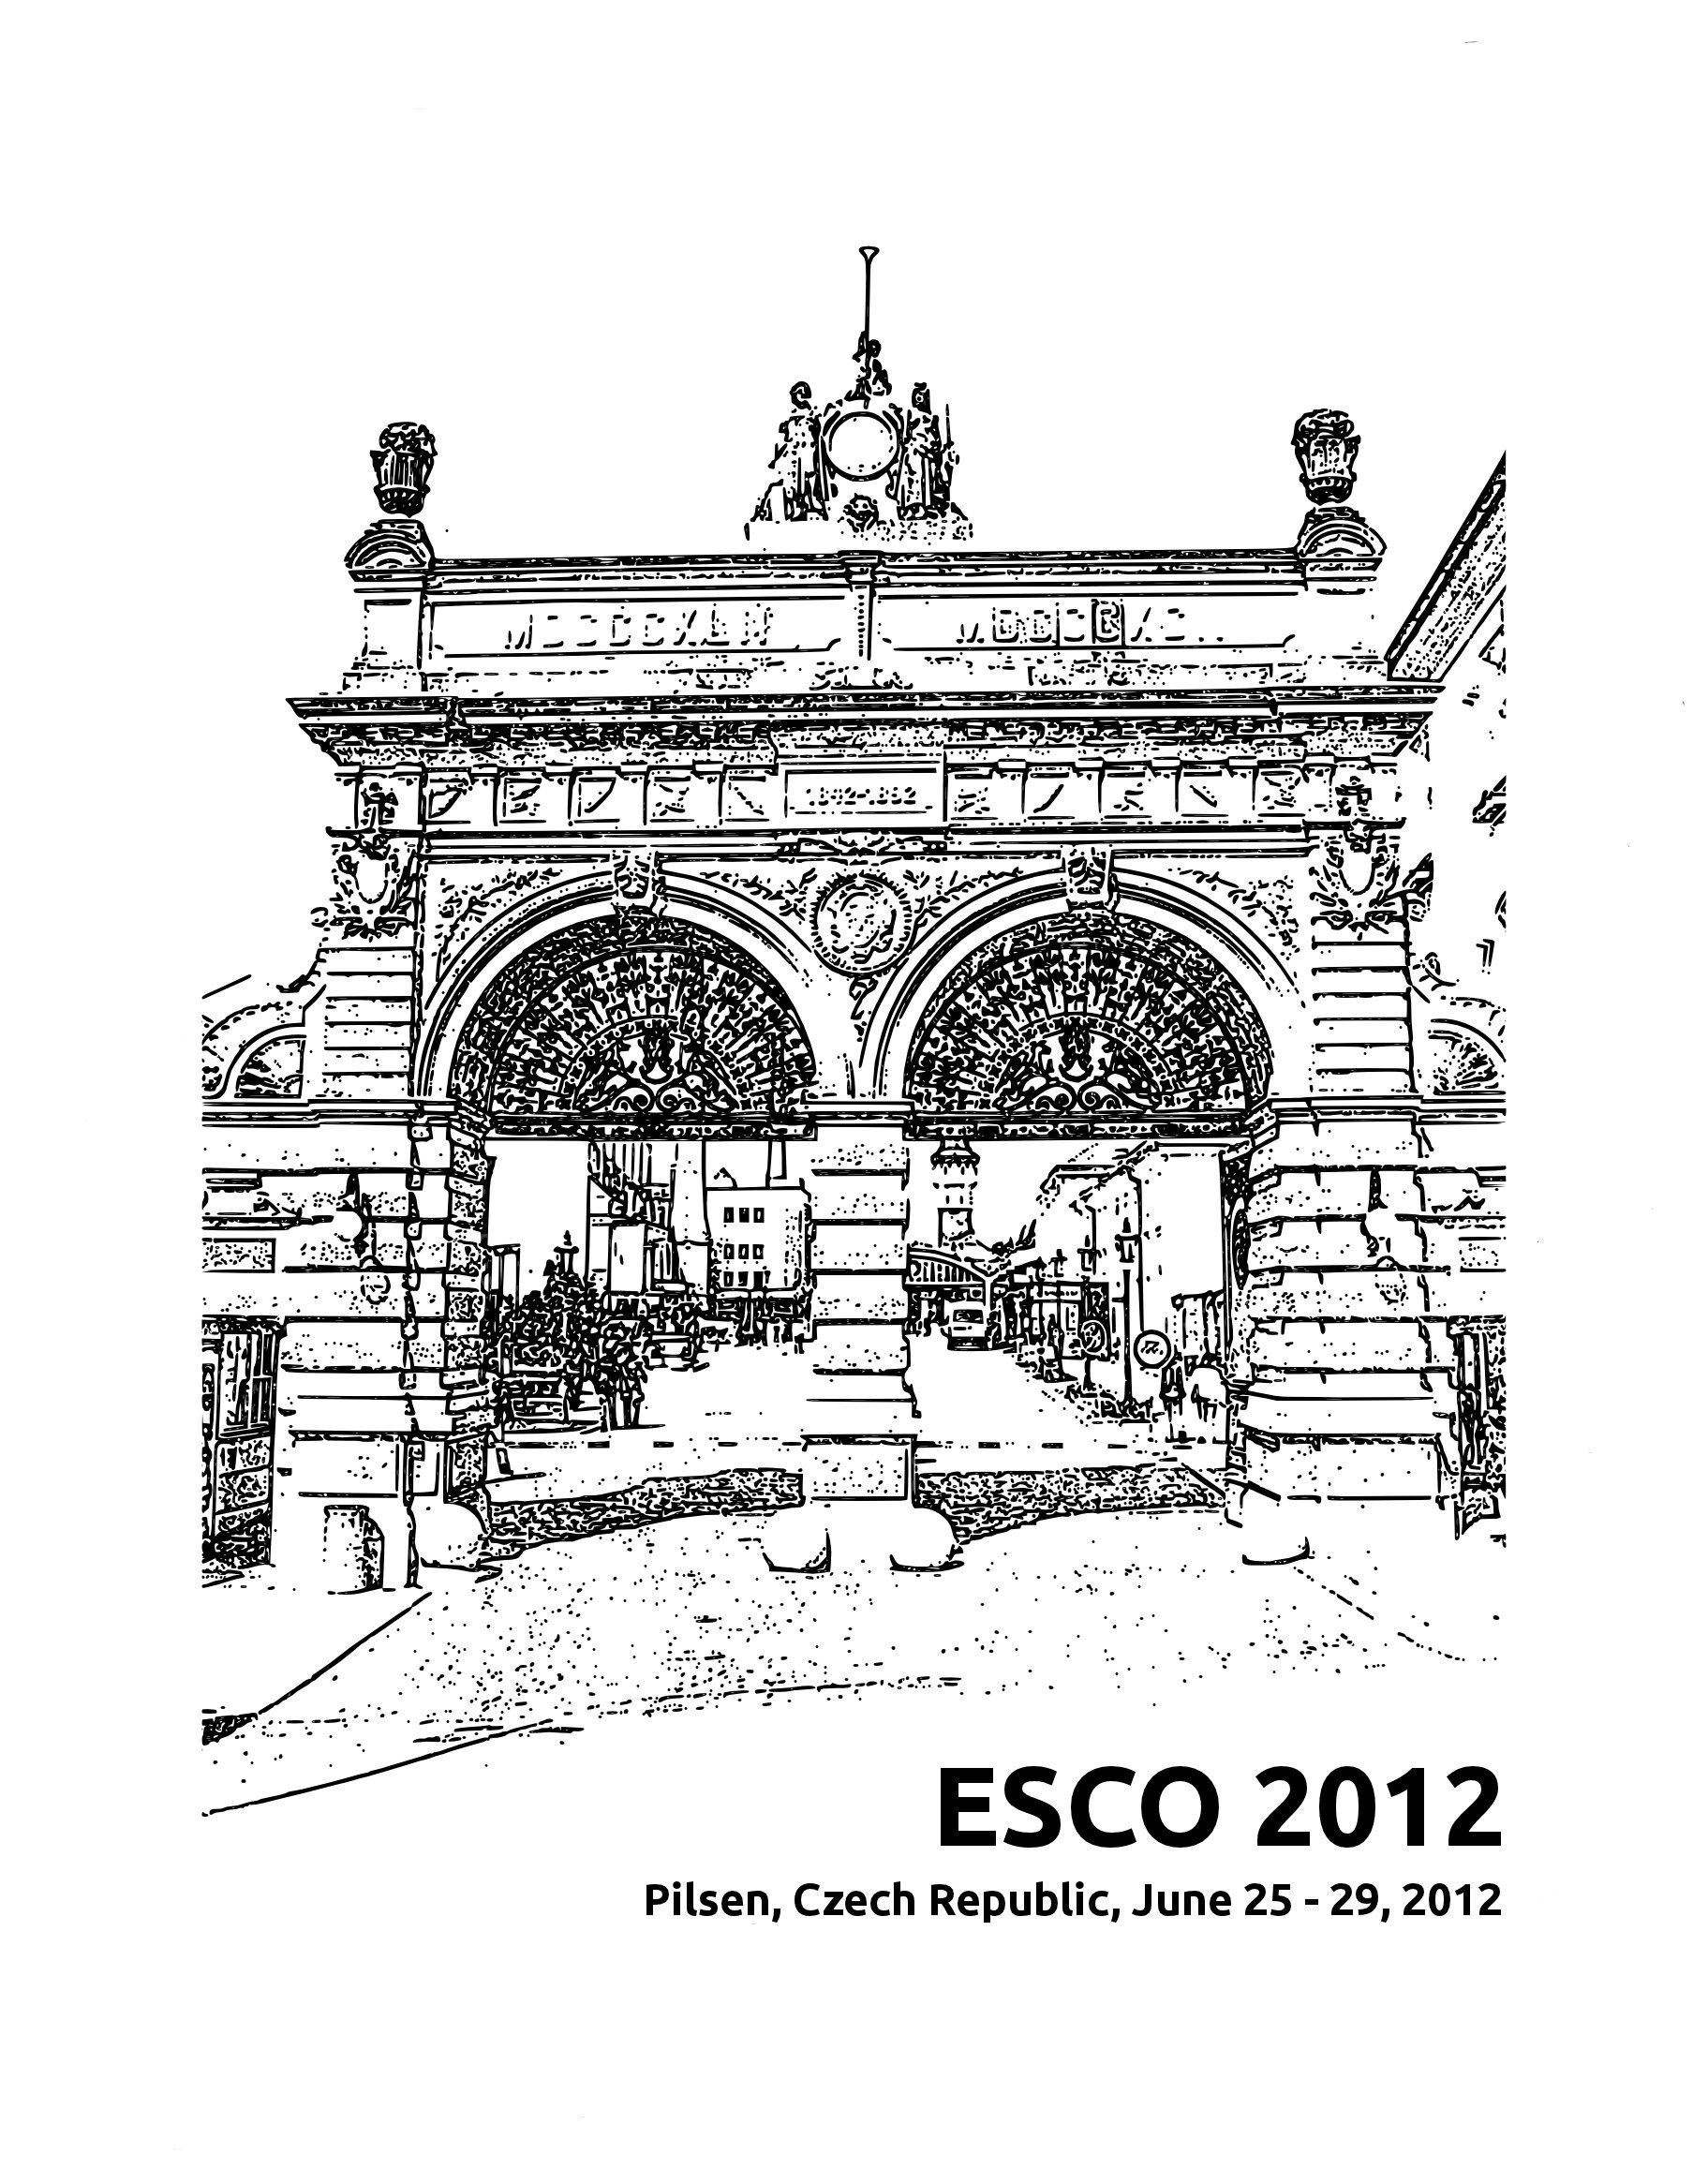
\includegraphics[width=\paperwidth,height=\paperheight]{background_new.jpg}%
\vfill
}}}

% BEGIN DOCUMENT
\begin{document}

% inputting background image
\AddToShipoutPicture{\BackgroundPic}

\vbox{}
\pagestyle{empty}

\newpage

\textwidth=15.5cm

\ClearShipoutPicture

\newpage

\section*{}%

\vspace*{60mm}
%ISBN 978-80-7043-898-5\\ \\
This is a joint publication of the University of Nevada (Reno, USA),
University of West Bohemia (Pilsen, Czech Republic), 
Czech Technical University (Prague, Czech Republic), 
Institute of Thermomechanics (Prague, Czech Republic), and
FEMhub Inc (Reno, USA).\\

\noindent
ESCO 2012 \\ 
3rd European Seminar on Computing\\

\noindent
\begin{tabular}{ll}
Editors: & Pavel Solin (University of Nevada, Institute of Thermomechanics) \\
 & Pavel Karban (University of West Bohemia) \\
 & Jaroslav Kruis (Czech Technical University) \\
Publisher: & University of West Bohemia \\
 & Univerzitn\'{i} 8, 306 14 Plze\u{n}\\
 & Czech Republic\\
Printed by: & Dragon Print, s.r.o \\
 & Klatovsk\'{a} 24, 301 00 Plze\u{n}\\
 & Czech Republic\\
Year: & 2012\\
\end{tabular}

\subsection*{Contact Information}

Mailing address:\\
ESCO 2012 Conference\\
FEMhub Inc.\\
5490 Twin Creeks Dr.\\
Reno, NV 89523\\
U.S.A. 

\noindent
E-mail: {\tt esco2012@femhub.com}\\
Web page: {\tt http://esco2012.femhub.com/}\\
Phone: 1-775-848-7892

\chapter*{\huge ESCO 2012}
\vspace{-5mm}
\normalsize   
\begin{center}
3rd European Seminar on Computing, 
Pilsen, Czech Republic,
June 25 - 29, 2012
\end{center}
\vspace{-3mm}

\section*{Main Thematic Areas}%

Multiphysics coupled problems; Higher-order computational methods
Computing with Python; GPU computing; Cloud computing.

\section*{Application Areas}%

Theoretical results as well as applications are welcome. Application areas include, but are not limited to: Computational electromagnetics, Civil engineering, Nuclear engineering, Mechanical engineering, Nonlinear dynamics, Fluid dynamics, Climate and weather modeling, Computational ecology, Wave propagation, Acoustics, Geophysics, Geomechanics and rock mechanics, Hydrology, Subsurface modeling, Biomechanics, Bioinformatics, Computational chemistry, Stochastic differential equations, Uncertainty quantification, and others.

\subsection*{Scientific Committee}%

%\hspace{4mm} 

\begin{itemize}
\item Valmor de Almeida (Oak Ridge National Laboratory, Oak Ridge, USA)
\item Zdenek Bittnar (Faculty of Civil Engineering, CTU Prague)
\item Alain Bossavit (Laboratoire de Genie Electrique de Paris, France)
\item John Butcher (Auckland University, New Zealand)
\item Antonio DiCarlo (University Roma Tre, Rome, Italy)
\item Ivo Dolezel (Czech Technical University, Prague, Czech Republic)
\item Stefano Giani (University of Nottingham, UK)
\item Glen Hansen (Sandia National Laboratories, Albuquerque, USA)
\item Pavel Karban (University of West Bohemia, Pilsen, Czech Republic)
\item Darko Koracin (Desert Research Institute, Reno, USA)
\item Dmitri Kuzmin (University of Erlangen-Nuremberg, Germany)
\item Stephane Lanteri (INRIA, Sophia-Antipolis, France)
\item Jichun Li (University of Nevada, Las Vegas, USA)
\item Shengtai Li (Los Alamos National Laboratory, Los Alamos, USA)
\item Alberto Paoluzzi (University Roma Tre, Rome, Italy)
\item Jean Ragusa (Texas A\&M University, College Station, USA)
\item Francesca Rapetti (University of Nice, France)
\item Sascha Schnepp (Technical University of Darmstadt, Germany)
\item Stefan Turek (Technical University of Dortmund, Germany)
\end{itemize}

\subsection*{Organizing Committee}

\begin{itemize}
\item Pavel Solin (University of Nevada, Reno \& Institute of Thermomechanics, Prague)
\item Pavel Karban  (University of West Bohemia, Pilsen)
\item Jaroslav Kruis (Czech Technical University, Prague)
\end{itemize}

\newpage
{\ }

\tableofcontents



%%%%%%%%%%%%%%%%%%%%%%%%%%%%%%%%%%%%%%%%%%%%%%%%%%%%%%%%%%%%%%%%%%%%%%%%%%%%%%%%%%%%%%%%%%%%%%%%%%%%%%%%%%%%%%%%%%%%%%%%%%%%%%%%%%%%%%%%%%%%%%%%%%%%%%%%%
\part{Abstracts of Keynote Lectures}

\pagestyle{plain}

\input baker.tex \newpage
\input butcher1.tex \newpage
\input gee.tex \newpage
\input mcinnes.tex \newpage
\input posey.tex \newpage

%--------------------------------------------------------------------------------------
\part{Abstracts of Contributed Lectures}

\input abed.tex \newpage
\input akgun.tex \newpage
\input alassar.tex \newpage
\input almag.tex \newpage
\input barash.tex \newpage
\input basting.tex \newpage
\input basting2.tex \newpage
%\input bazin.tex \newpage            % NEMA ABSTRAKT
\input benesl.tex \newpage
\input bittl.tex \newpage
\input brambilla.tex \newpage
\input braun.tex \newpage
\input butcher2.tex \newpage
\input chleb.tex \newpage
\input ciobanescu.tex \newpage
\input cimr.tex \newpage
\input dagostino.tex \newpage
\input descombes.tex \newpage
\input dhee.tex \newpage
\input dicarlo.tex \newpage
\input dicarlo2.tex \newpage
\input dimier.tex \newpage
\input emans.tex \newpage
\input engstrom.tex \newpage
\input fuka.tex \newpage
\input fernandez.tex \newpage
\input frydrych.tex \newpage
\input furma.tex \newpage
\input furst.tex \newpage
\input gedicke.tex \newpage
\input georgiev.tex \newpage
\input giani.tex \newpage
\input giani2.tex \newpage
\input golab.tex \newpage
\input grubisic.tex \newpage
\input gugala.tex \newpage
\input haas.tex \newpage
\input hakula.tex \newpage
\input halama.tex \newpage
\input hall.tex \newpage
\input han.tex \newpage
\input hanus.tex \newpage
\input harbrecht.tex \newpage
\input hasnedl.tex \newpage
\input havl.tex \newpage
\input hijazi.tex \newpage
\input hokr.tex \newpage
\input horenkamp.tex \newpage
\input holzbecher.tex \newpage
\input horng.tex \newpage
\input junge.tex \newpage
\input karacor.tex \newpage
\input karban.tex \newpage
\input kesle.tex \newpage
\input klimach.tex \newpage
\input kolditz.tex \newpage
\input koltai.tex \newpage
\input korek.tex \newpage
\input korous.tex \newpage
\input kosik.tex \newpage
\input kotlan.tex \newpage
\input koudela.tex \newpage
\input krejci.tex \newpage
\input kropik.tex \newpage
\input kruis.tex \newpage
\input kucera.tex \newpage
\input kucerova.tex \newpage
\input kuraz.tex \newpage
\input kus.tex \newpage
\input lang.tex \newpage
\input lebrun.tex \newpage
\input leps.tex \newpage
\input leubner.tex \newpage
\input lev.tex \newpage
\input liebmann.tex \newpage
\input lilie.tex \newpage
\input louda.tex \newpage
\input mangu.tex \newpage
\input matyka.tex \newpage
\input metsch.tex \newpage
\input moeller.tex \newpage
\input moiola.tex \newpage
\input morales.tex \newpage
\input mussa.tex \newpage
\input neic.tex \newpage
\input neumaier.tex \newpage
\input niege.tex \newpage
\input norton.tex \newpage
\input norton2.tex \newpage
\input nunez.tex \newpage
\input ouden.tex \newpage
\input padberg.tex \newpage
\input paprok.tex \newpage
%\input panek.tex \newpage             % NEMA ABSTRACT
\input patterson.tex \newpage
\input podhai.tex \newpage
\input poko.tex \newpage
\input poriz.tex \newpage
\input principe.tex \newpage
\input prokop.tex \newpage
\input rapetti.tex \newpage
\input rieger.tex \newpage
\input roemer.tex \newpage
\input rohan.tex \newpage
\input rosic.tex \newpage
\input sawi.tex \newpage
\input schieche.tex \newpage
\input schmidt.tex \newpage
\input schnepp.tex \newpage
\input segeth.tex \newpage
\input sehnalova.tex \newpage
\input sistek.tex \newpage
\input solin.tex \newpage
\input soto.tex \newpage
\input soto2.tex \newpage
\input starzynski.tex \newpage
\input stork.tex \newpage
\input svacek.tex \newpage
\input sykora.tex \newpage
\input szabo.tex \newpage
\input tezer.tex \newpage
\input trommler.tex \newpage
\input ullmann.tex \newpage
\input urev.tex \newpage
\input urev2.tex \newpage
\input valkonen.tex \newpage
\input vonka.tex \newpage
\input voracek.tex \newpage
\input weber.tex \newpage
\input zander.tex \newpage
\input zaspel.tex \newpage
\input zhao.tex \newpage
\input zubov.tex \newpage






%--------------------------------------------------------------------------------------
%\newpage


%\part{List of Participants}

%\input addresses.tex
%\input esco_users.tex

%--------------------------------------------------------------------------------------
%--------------------------------------------------------------------------------------
%--------------------------------------------------------------------------------------


\end{document}
